\chapter{Problem Formulation}
\label{cha:problem_formulation}

This chapter introduces the formal model that underpins this thesis. We consider a generalization of the standard kidney exchange framework, where each patient may be associated with more than one donor. We begin by reviewing the conventional patient-donor pair model and then extend it to accommodate the setting with multiple donors per patient. We subsequently define a series of algorithmic problems that emerge in this multi-donor context. These problems depart from classical kidney exchange formulations and can be interpreted from multiple perspectives.%, including structured graph matching, weighted set packing, and integer programming. This chapter establishes the theoretical foundation for the complexity analysis, algorithm design, and experimental evaluation presented in the subsequent chapters.

\section{Overview of the Model}

We begin by reviewing a model which is commonly used in kidney exchange literature. In the model, each node represents a \textit{patient-donor pair}, and each directed edge indicates that the donor in the source node is compatible with the patient in the target node. This results in an unweighted directed graph $G = (V, E)$. Depending on the specific problem setting (such as restrictions on the length of allowed exchange cycles) this formulation leads to different variants of graph matching problems. In general, however, the objective is to find disjoint exchange cycles that include the maximum number of patients.

Extending the model to the version where each patient is associated with multiple \textit{alternative donors} is straightforward. In this extension, each patient along with all his associated proxy donors is still represented as a single node in the graph. The compatibility edges are then defined such that a directed edge from node $u$ to node $v$ exists if any of the donors associated with patient $u$ is compatible with the patient in node $v$. This preserves the structure of the original graph as a directed graph $G = (V, E)$, but with a potentially denser set of edges due to the increased number of donor-patient compatibility possibilities. This setting is then identical to the standard patient-donor pair KE problem: the objective is still to find disjoint exchange cycles in a directed compatibility graph.

A more general scenario arises if we allow a patient to receive a kidney while all of their associated donors are permitted to donate simultaneously. We call this model \textit{multiple donors} model. How this model relates to other kidney exchange models is shown in \autoref{fig:models_hierarchy}. In this case, one of the donors may participate in an exchange cycle as usual, while other donor initiate a donation chains, effectively increasing the total number of transplants.




\begin{figure}
    \centering
    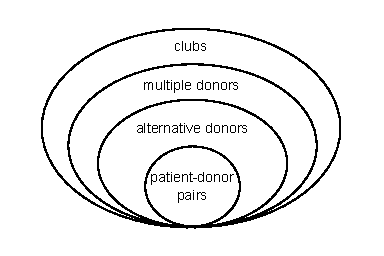
\includegraphics{data/models_hierarchy.pdf}
    \caption[Hierarchy of kidney exchange models]{Hierarchy of kidney exchange models. Each successive set is a superset of the previous: patient-donor pairs form the core, extended by alternative donors, multiple donors, and finally clubs briefly mentioned in \autoref{sec:background_and_motivation}.}
    \label{fig:models_hierarchy}
\end{figure}

In such settings, we observe that allowing chains to follow cycles can only improve social welfare—it never reduces the total number of transplants compared to \textit{patient-donor pairs} model. Moreover, this problem deviates from the classical graph matching framework: it is no longer a pure matching problem.

Finally, we note that it is now possible for one donor to participate in a cycle while the second donor from the same patient initiates or joins a chain. This creates a structural asymmetry in the problem. A general graph representation (i.e. grouping patient and donor into one node) is no longer sufficient. Instead, we need to explicitly distinguish between patients and donors in the model to accurately capture the structure and constraints of the problem. An example of a graph with a patient having two proxy donors is shown in \autoref{fig:multiple_model_example}.

The \textit{multiple donors} model is a generalization of the \textit{alternative donors} model and therefore also accommodates groups consisting of a patient with alternative proxy donors. This case is handled in the same way as in the \textit{alternative donors} model—the donors are merged into a single node, as shown in \autoref{fig:alternative_model_example}.

Throughout the thesis, we will use the \textit{multiple-donors} model—that is, the one that distinguishes between node types. We also restrict the model to the case where each patient have at most two proxy donors. In the diagrams, patients will be represented as circles and donors as squares. Compatibility edges will be represented as solid arrows and proxy edges as dotted arrows.

\begin{figure}[htbp]
  \centering
  \begin{minipage}[t]{0.48\textwidth}
    \centering
    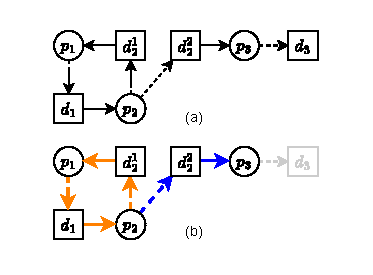
\includegraphics{data/multiple_model_example.pdf}
    \caption[An example of a graph with a patient having two donors]{\textbf{(a)} is an example of a graph where a patient has two proxy donors. \textbf{(b)} illustrates that this allows the model to select the cycle $(p_2 \rightarrow d_2^1 \rightarrow p_1 \rightarrow d_1 \rightarrow p_2)$ (in orange) and the chain $(p_2 \rightarrow d_2^2 \rightarrow p_3)$ (in blue).}
    \label{fig:multiple_model_example}
  \end{minipage}
  \hfill
  \begin{minipage}[t]{0.48\textwidth}
    \centering
    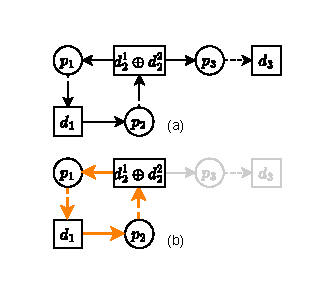
\includegraphics{data/alternative_model_example.pdf}
    \caption[An example of a graph with a patient having two alternative donors]{\textbf{(a)} is an example of a graph where a patient has two alternative proxy donors. \textbf{(b)} shows that only the cycle $(p_2 \rightarrow d_2^1 \rightarrow p_1 \rightarrow d_1 \rightarrow p_2)$ is selected in the solution.}
    \label{fig:alternative_model_example}
  \end{minipage}
\end{figure}

\section{Formal Definitions}

We formalize the \textit{multiple donors} model as a directed graph $G = (V, E)$, where the vertex set $V = P \cup D$ consists of two disjoint subsets: a set of patients $P$ and a set of donors $D$. The edge set $E$ is partitioned into two disjoint subsets, $E = E_{\mathrm{proxy}} \cup E_{\mathrm{compatible}}$, defined as follows:
\begin{itemize}
    \item The set of \textit{proxy edges} $E_{\mathrm{proxy}} \subseteq P \times D$ contains an edge $(p, d)$ if donor $d \in D$ is a proxy donor of patient $p \in P$.
    \item The set of \textit{compatibility edges} $E_{\mathrm{compatible}} \subseteq D \times P$ contains an edge $(d, p)$ if donor $d \in D$ is compatible with patient $p \in P$.
\end{itemize}

Each donor is a proxy for exactly one patient, and each patient has at most two proxy donors. We assume that no donor is compatible with their own associated patient, i.e., for all $(p, d) \in E_{\mathrm{proxy}}$, we have $(d, p) \notin E_{\mathrm{compatible}}$.
% If a patient reports his donors as \textit{alternative donors}, those donors are modeled as a single donor node. This node represents the whole set of alternative donors, and a compatibility edge exists if any of them is compatible with a patient.

A solution is a subgraph $G^{\mathrm{*}} = (V, E^{\mathrm{*}})$ with $E^{\mathrm{*}} \subseteq E$ satisfying the following constraints:
\begin{enumerate}
    \item \textbf{Patient receives at most one kidney:}  
    Each patient receives at most one kidney from a compatible donor:  
    \[
        \forall p \in P, \quad \left| \{ d \in D : (d, p) \in E^{\mathrm{*}}_{\mathrm{compatible}} \} \right| \le 1.
    \]
    \item \textbf{Donor donates only if proxy patient is matched:}  
    A donor $d$ may donate a kidney for some patient $p$ if and only if his associated patient $p'$ also receives a compatible kidney, i.e.,  
    \[
        (d, p) \in E^{\mathrm{*}}_{\mathrm{compatible}} \iff (p', d) \in E_{\mathrm{proxy}} \text{ and } \exists (d', p') \in E^{\mathrm{*}}_{\mathrm{compatible}}.
    \]
\end{enumerate}

As mentioned in ~\autoref{cha:preliminaries}, our goal is to design algorithms for this model that ideally satisfy the following three properties:  
(i) truthfulness (DSIC),  
(ii) maximization of social welfare, and  
(iii) computational efficiency.

\section{Problems Variants}

The model introduced above captures the essential structure of multi-donor kidney exchange and donation. We now build upon this model to define specific algorithmic problems under various settings. The remainder of this paper will focus on analyzing and solving these problems.

As a starting point, consider the most general setting, where no restrictions are imposed on the length of exchange cycles or donation chains. Given a directed graph $G = (V = P \cup D, E)$, all subsets of edges that satisfy the feasibility constraints described earlier are considered valid solutions. We refer to this formulation as the \textit{Unbounded Multi-Donor Exchange Problem}.

We then consider a more constrained version, where limits are placed on the maximum allowed lengths of cycles and chains. Specifically, in the \textit{$n$-Cycle $m$-Chain Problem}, only subsets in which all cycles have length at most $n$ and all chains have length at most $m$ are considered valid. Here, the length refers to the number of compatible edges the cycle or the chain contains. Returning to the example from \autoref{fig:multiple_model_example}, the cycle has length $2$ and the chain has length $1$.



\section{Alternative Interpretations}

The problem we consider has a structured, graph-like nature. This subsection explores how our model connects to classical problem frameworks, providing alternative perspectives that inform both algorithmic design and empirical evaluation.

\subsection{Weighted Set Packing}

\label{pro:weighted_set_packing}

One useful interpretation frames our problem as a special case of the \emph{weighted set packing} problem. Each feasible subset corresponds to a valid exchange (either a cycle or a cycle followed by chain(s)) with the constraint that no individual (patient or donor) can appear in more than one subset. The objective is to select a collection of disjoint subsets that maximizes the total number of patients matched, which defines the weight of each subset. We adopt this perspective in the design of a randomized mechanism presented in \autoref{cha:approximation}.




\subsection{Integer Linear Program Formulation}
Additionally, our problem can be formulated as an \emph{integer linear program (ILP)}. In the experimental section \autoref{cha:Experiments}, we implement and solve such an ILP to evaluate the practical effectiveness and scalability of our approach.

%Following is integer linear program formulation for \textit{2-cycle 1-chain kidney exchange problem}, which will be used in \autoref{cha:Experiments}.

Let:
\begin{itemize}
    \item $P$ be the set of all patients.
    \item $D$ be the set of all donors.
    \item $Cycles$ be a set of all possible 2-cycles formed by patients and donors from $P$ and $D$.
    \item $Chains$ be a set of all possible chains of length 1 starting from a cycle.
\end{itemize}

The ILP formulation of \textit{2-cycle 1-chain kidney exchange problem} is given as:
\begin{align*}
\max\quad & \sum_{c \in \text{Cycles}} 2x_c + \sum_{e \in \text{Chains}} x_e \\
\text{s.t.}\quad 
 (1)\: & \sum_{\substack{c \in \text{Cycles} \\ d \in c}} x_c + \sum_{\substack{e \in \text{Chains} \\ e.\text{start} = d}} x_e \le 1 && \forall d \in D \\
(2)\: & \sum_{\substack{c \in \text{Cycles} \\ p \in c}} x_c + \sum_{\substack{e \in \text{Chains} \\ e.\text{end} = p}} x_e \le 1 && \forall p \in P \\
(3)\: & \sum_{\substack{c \in \text{Cycles} \\ p_i \in c}} x_c \ge x_e && \forall e = (d_i, p_j),\ i \ne j \\
& x_c \in \{0, 1\} && \forall c \in \text{Cycles} \\
& x_e \in \{0, 1\} && \forall e \in \text{Chains}
\end{align*}
\noindent
(1) and (2) ensures that every donor and patient are selected in at most one cycle or chain.
(3) ensures that a chain is started from a donor which proxy patient is already selected in a cycle. This also ensures that length of the chain is 1. The objective is to select set of cycles and chains that maximize the number of matched patients.

%%% Local Variables:
%%% mode: latex
%%% TeX-master: "../ClassicThesis"
%%% ispell-dictionary: "british" ***
%%% fill-column: 76 ***
%%% End:
